%% For double-blind review submission, w/o CCS and ACM Reference (max submission space)
%\documentclass[acmsmall,review,anonymous]{acmart}\settopmatter{printfolios=true,printccs=false,printacmref=false}
%% For double-blind review submission, w/ CCS and ACM Reference
%\documentclass[acmsmall,review,anonymous]{acmart}\settopmatter{printfolios=true}
%% For single-blind review submission, w/o CCS and ACM Reference (max submission space)
%\documentclass[acmsmall,review]{acmart}\settopmatter{printfolios=true,printccs=false,printacmref=false}
%% For single-blind review submission, w/ CCS and ACM Reference
%\documentclass[acmsmall,review]{acmart}\settopmatter{printfolios=true}
%% For final camera-ready submission, w/ required CCS and ACM Reference
\documentclass[acmsmall, review]{acmart}\settopmatter{}

%% Journal information
%% Supplied to authors by publisher for camera-ready submission;
%% use defaults for review submission.
\acmJournal{PACMPL}
\acmVolume{2}
\acmNumber{ICFP} % CONF = POPL or ICFP or OOPSLA
\acmArticle{1}
\acmYear{2018}
\acmMonth{9}
\acmDOI{10.1145/nnnnnnn.nnnnnnn}
\startPage{1}

%% Copyright information
%% Supplied to authors (based on authors' rights management selection;
%% see authors.acm.org) by publisher for camera-ready submission;
%% use 'none' for review submission.
% TODO: Which one?
%\setcopyright{none}
%\setcopyright{acmcopyright}
\setcopyright{acmlicensed}
%\setcopyright{rightsretained}
%\copyrightyear{2018}           %% If different from \acmYear

%% Bibliography style
\bibliographystyle{ACM-Reference-Format}
%% Citation style
%% Note: author/year citations are required for papers published as an
%% issue of PACMPL.
\citestyle{acmauthoryear}   %% For author/year citations


%%%%%%%%%%%%%%%%%%%%%%%%%%%%%%%%%%%%%%%%%%%%%%%%%%%%%%%%%%%%%%%%%%%%%%
%% Note: Authors migrating a paper from PACMPL format to traditional
%% SIGPLAN proceedings format must update the '\documentclass' and
%% topmatter commands above; see 'acmart-sigplanproc-template.tex'.
%%%%%%%%%%%%%%%%%%%%%%%%%%%%%%%%%%%%%%%%%%%%%%%%%%%%%%%%%%%%%%%%%%%%%%


%% Some recommended packages.
\usepackage{booktabs}   %% For formal tables:
                        %% http://ctan.org/pkg/booktabs
\usepackage{subcaption} %% For complex figures with subfigures/subcaptions
%% http://ctan.org/pkg/subcaption

\usepackage[utf8]{inputenc}
\usepackage[T1]{fontenc}
\usepackage[scaled=0.85]{beramono}
\usepackage{amsmath}
\usepackage{amssymb}
\usepackage{xcolor,colortbl}
\usepackage{url}
\usepackage{listings}
\usepackage{paralist}
\usepackage{wrapfig}
\usepackage{enumitem}
\usepackage{multicol}
\usepackage{flushend}
\usepackage{tikz}

\usetikzlibrary{arrows,chains,matrix,positioning,scopes}
\makeatletter
\tikzset{join/.code=\tikzset{after node path={%
\ifx\tikzchainprevious\pgfutil@empty\else(\tikzchainprevious)%
edge[every join]#1(\tikzchaincurrent)\fi}}}
\makeatother

\tikzset{>=stealth',every on chain/.append style={join},
         every join/.style={->}}
\tikzstyle{labeled}=[execute at begin node=$\scriptstyle,
   execute at end node=$]

% ----- listings

\definecolor{ckeyword}{HTML}{7F0055}
\definecolor{ccomment}{HTML}{3F7F5F}
\definecolor{cstring}{HTML}{2A0099}

\lstdefinelanguage{Scala}%
{morekeywords={abstract,%
  sealed,%
  case,catch,char,class,%
  def,else,extends,final,finally,for,%
  if,import,implicit,%
  match,module,%
  new,null,undefined,%
  fun,array,
  override,%
  package,private,protected,public,%
  for,public,return,super,%
  this,throw,trait,try,type,%
  val,var,%
  with,while,%
  let,skip,assert,then,fst,snd,root,idx,sum,prod,exists,forall,%
  yield%
  },%
  sensitive,%
  moredelim=*[il][\bfseries]{\#\#\ },
  morecomment=[l]//,%
  morecomment=[s]{/*}{*/},%
  morestring=[b]",%
%  morestring=[b]',%
  showstringspaces=false%
}[keywords,comments,strings]%

\lstset{language=Scala,%
  mathescape=true,%
%  columns=[c]fixed,%
%  basewidth={0.5em, 0.40em},%
%  aboveskip=5pt,%\smallskipamount,
%  belowskip=5pt,%\negsmallskipamount,
  lineskip=0pt,
  basewidth={0.54em, 0.4em},%
%  backgroundcolor=\color{listingbg},
  basicstyle=\footnotesize\ttfamily,
  keywordstyle=\keywordstyle,
  commentstyle=\commentstyle,
  stringstyle=\stringstyle,
%  xleftmargin=0.5cm
  literate={-->}{{$\to$}}3 
           {->}{{$\mapsto$}}3 
           {=>}{{$\Rightarrow$}}2 
           {|-}{{$\ts$}}2 
           %{fun}{{$\lambda$}}1 
           {idx}{{$\#$}}1 
           %{sum}{{$\Sigma$}}1 
           {array(}{{$\langle.\rangle$(}}3 
           %{[[}{{$[\![$}}1
           %{]]}{{$]\!]$}}1
           %{…}{{$\!...$}}1 
}

\definecolor{listingbg}{RGB}{240, 240, 240}

\newcommand{\commentstyle}[1]{\color{ccomment}\itshape{#1}}
\newcommand{\keywordstyle}[1]{\color{ckeyword}\bfseries{#1}}
\newcommand{\stringstyle}[1]{\color{cstring}\bfseries{#1}}

\lstnewenvironment{listing}{\lstset{language=Scala}}{}
\lstnewenvironment{listingtiny}{\lstset{language=Scala,basicstyle=\scriptsize\ttfamily}}{}

\newcommand{\code}[1]{\lstinline[language=Scala,columns=fixed,basicstyle=\ttfamily]|#1|}


\newcommand{\IMP}[0]{\texttt{IMP}}
\newcommand{\FUN}[0]{\texttt{FUN}}

\newcommand{\TOOL}[0]{\texttt{SIGMA}}



% ----- packed items, so we don't waste space
\newenvironment{sitemize}{
\begin{itemize}
  \setlength{\itemsep}{1pt}
  \setlength{\parskip}{0pt}
  \setlength{\parsep}{0pt}
}{\end{itemize}}

\newenvironment{senumerate}{
\begin{enumerate}
  \setlength{\itemsep}{1pt}
  \setlength{\parskip}{0pt}
  \setlength{\parsep}{0pt}
}{\end{enumerate}}

\newcommand{\mypar}[1]{{\bf #1.}}

% ----- formal

%\newcommand{\judgement}[2]{{\bf #1} \hfill #2}
%\newcommand{\den}[1]{$\left\llbracket$\;#1\;$\right\rrbracket$}
\newcommand{\den}[1]{\llbracket~#1~\rrbracket}

%\newcommand{\ts}{\,\vdash\,}
\newcommand{\evalsto}{\Downarrow}

\newcommand{\mbind}{\;{\small{\texttt{>>}\hspace{-0.3pt}\raisebox{-0.15pt}{\texttt{=}}}}\;}

%\newcommand{\mbind}{{\small{\texttt{>>}\hspace{-1.7pt}\raisebox{-0.15pt}{\texttt{=}}}}}

\newcommand{\rref}[1]{\textsc{(#1)}}

% ----- comments and todo

\newcommand{\note}[1]{{\color{red}[#1]}}
\newcommand{\todo}[1]{\note{TODO: #1}}

\newcommand{\silent}[1]{}



\begin{document}

%% Title information
\title{Refunctionalization of Abstract Abstract Machines (Functional Pearl)}         %% [Short Title] is optional;
                                        %% when present, will be used in
                                        %% header instead of Full Title.
%\titlenote{with title note}             %% \titlenote is optional;
                                        %% can be repeated if necessary;
                                        %% contents suppressed with 'anonymous'
\subtitle{Filling the Gap Between Abstract Abstract Machines and Abstract Definitional Interpreters}        %% \subtitle is optional
%\subtitlenote{with subtitle note}       %% \subtitlenote is optional;
                                        %% can be repeated if necessary;
                                        %% contents suppressed with 'anonymous'


%% Author information
%% Contents and number of authors suppressed with 'anonymous'.
%% Each author should be introduced by \author, followed by
%% \authornote (optional), \orcid (optional), \affiliation, and
%% \email.
%% An author may have multiple affiliations and/or emails; repeat the
%% appropriate command.
%% Many elements are not rendered, but should be provided for metadata
%% extraction tools.

%% Author with single affiliation.
\author{Guannan Wei}
%\authornote{with author1 note}          %% \authornote is optional;
                                        %% can be repeated if necessary
% TODO: Register a OrcID
%\orcid{nnnn-nnnn-nnnn-nnnn}             %% \orcid is optional
\affiliation{
  \position{Position1}
  \department{Department of Computer Science}              %% \department is recommended
  \institution{Purdue University}            %% \institution is required
  \streetaddress{305 N. University Street}
  \city{West Lafayette}
  \state{IN}
  \postcode{47907}
  \country{USA}                    %% \country is recommended
}
\email{wei220@purdue.edu}          %% \email is recommended

\author{James Decker}
%\authornote{with author1 note}          %% \authornote is optional;
                                        %% can be repeated if necessary
%\orcid{nnnn-nnnn-nnnn-nnnn}             %% \orcid is optional
\affiliation{
  \position{Position1}
  \department{Department of Computer Science}              %% \department is recommended
  \institution{Purdue University}            %% \institution is required
  \streetaddress{305 N. University Street}
  \city{West Lafayette}
  \state{IN}
  \postcode{47907}
  \country{USA}                    %% \country is recommended
}
\email{decker31@purdue.edu}          %% \email is recommended

\author{Tiark Rompf}
%\authornote{with author1 note}          %% \authornote is optional;
                                        %% can be repeated if necessary
%\orcid{nnnn-nnnn-nnnn-nnnn}             %% \orcid is optional
\affiliation{
  \position{Position1}
  \department{Department of Computer Science}              %% \department is recommended
  \institution{Purdue University}            %% \institution is required
  \streetaddress{305 N. University Street}
  \city{West Lafayette}
  \state{IN}
  \postcode{47907}
  \country{USA}                    %% \country is recommended
}
\email{tiark@purdue.edu}          %% \email is recommended

\iffalse
%% Author with two affiliations and emails.
\author{First2 Last2}
\authornote{with author2 note}          %% \authornote is optional;
                                        %% can be repeated if necessary
\orcid{nnnn-nnnn-nnnn-nnnn}             %% \orcid is optional
\affiliation{
  \position{Position2a}
  \department{Department2a}             %% \department is recommended
  \institution{Institution2a}           %% \institution is required
  \streetaddress{Street2a Address2a}
  \city{City2a}
  \state{State2a}
  \postcode{Post-Code2a}
  \country{Country2a}                   %% \country is recommended
}
\email{first2.last2@inst2a.com}         %% \email is recommended
\affiliation{
  \position{Position2b}
  \department{Department2b}             %% \department is recommended
  \institution{Institution2b}           %% \institution is required
  \streetaddress{Street3b Address2b}
  \city{City2b}
  \state{State2b}
  \postcode{Post-Code2b}
  \country{Country2b}                   %% \country is recommended
}
\email{first2.last2@inst2b.org}         %% \email is recommended
\fi

\lstMakeShortInline[keywordstyle=,%
                    flexiblecolumns=false,%
                    %basewidth={0.56em, 0.52em},%
                    mathescape=false,%
                    basicstyle=\tt]@

%% Abstract
%% Note: \begin{abstract}...\end{abstract} environment must come
%% before \maketitle command
\begin{abstract}
  Abstracting abstract machines (AAM) is a systematic methodology for constructing 
  abstract interpreters that are derived from concrete small-step abstract machines.
  Recent progress applies the same idea on definitional interpreters, and obtains
  big-step abstract definitional interpreters (ADI) written in monadic style.
  Yet, the relations between small-step abstracting abstract machines and big-step 
  abstracting definitional interpreters are not well studied.

  In this paper, we show their functional correspondence and how to syntactically 
  transform small-step abstract abstract machines into big-step abstract definitional
  interpreters.
  The transformations include linearization, lightweight fusion, disentanglement, 
  refunctionalization, and finally back to direct-style with delimited control operators. 
  Linearization expresses nondeterministic choices by first-order data types, 
  after which refunctionalization transforms the data type representing continuations
  into higher-order functions.
  Following the idea that in deterministic languages, reduction contexts of reduction
  semantics are defunctionalized continuations, we further apply this idea to nondeterministic
  AAM -- its reduction contexts are refunctionalized to extended continuation-passing style.
  
  All transformations properly handle the collecting semantics and the nondeterminism 
  of abstract interpretation. Remarkably, we reveal how precise call/return matching in 
  control-flow analysis can be obtained by refunctionalizing a small-step abstract abstract 
  machine with proper caching.
\end{abstract}

% TODO: Update CCS
%% 2012 ACM Computing Classification System (CSS) concepts
%% Generate at 'http://dl.acm.org/ccs/ccs.cfm'.
\begin{CCSXML}
<ccs2012>
  <concept>
    <concept_id>10011007.10011006.10011008</concept_id>
    <concept_desc>Software and its engineering~General programming languages</concept_desc>
    <concept_significance>500</concept_significance>
  </concept>
  <concept>
    <concept_id>10003456.10003457.10003521.10003525</concept_id>
    <concept_desc>Social and professional topics~History of programming languages</concept_desc>
    <concept_significance>300</concept_significance>
  </concept>
</ccs2012>
\end{CCSXML}
\ccsdesc[500]{Software and its engineering~General programming languages}
\ccsdesc[300]{Social and professional topics~History of programming languages}
%% End of generated code


%% Keywords
%% comma separated list
\keywords{refunctionalization, abstract machines, abstract interpretation}  %% \keywords are mandatory in final camera-ready submission


%% \maketitle
%% Note: \maketitle command must come after title commands, author
%% commands, abstract environment, Computing Classification System
%% environment and commands, and keywords command.
\maketitle


\section{Introduction}

Defining a language by building an interpreter for it can be traced to the very
early days of programming languages research \cite{landin1966next, Reynolds:72}.
Nowadays, even an undergraduate student in computer science is able to build toy 
languages through interpreters.
But building a sound abstract interpreter remained an esoteric and difficult task 
until very recently.

\citeauthor{van2012systematic} proposed the Abstracting Abstract Machines (AAM) 
methodology which provides a recipe for constructing sound abstract interpreters 
for higher-order functional languages from concrete abstract machines 
~\cite{van2012systematic, van2010abstracting}.
Given a concrete small-step abstract machine (e.g. the CESK machine, Krivine's 
machine, etc.), by allocating continuations in the store and bounding both the 
value addresses and continuation addresses to be finite, we obtain an abstract 
interpreter with a finite state space which can be used for performing sound 
static analysis.
One can further instantiate different polyvariant control-flow analyses by using
different address allocators \cite{Gilray:2016:ACP:2951913.2951936}.

Applying the same idea to big-step definitional interpreters, \citeauthor{darais2017abstracting}
built abstract definitional interpreters (ADI) that are written in monadic style 
\cite{darais2017abstracting}. One of the advantages of a monadic interpreter is 
that it is modular and composable. By changing the underlying monads, the definition
of the interpreter is not modified, but we can recover different semantics, including
the concrete semantics and various abstract semantics such as context-sensitivity and
abstract garbage collection \cite{Sergey:2013:MAI:2491956.2491979}.

Broadly speaking, abstract abstract machines and abstract definitional interpreters are
different forms of abstract interpreters. They are obtained by applying a combination 
of abstractions to their concrete counterparts, abstract machines and definitional 
interpreters, respectively. An interesting question, and the subject of this paper, is 
how we can interderive these abstract semantic artifacts from the respective other one.

In the concrete world, the relations among reduction semantics, abstract machines,
definitional interpreters, and monadic interpreters have been intensively studied by
Danvy and his collaborators \cite{Ager:2003:FCE:888251.888254, Danvy:2001:DW:773184.773202,
danvy2004refocusing, Danvy:2008:DIP:1411204.1411206, AGER2004223, ager2005functional, 
Danvy:2006:RW:2171265.2171268, danvy2009towards, biernacka2009towards}.
The concrete abstract machines implement structural operational semantics in 
continuation-passing style, where the reduction contexts are defunctionalized continuations.
One can derive definitional interpreters by refunctionalizing the reduction contexts of 
abstract machines, and by defunctionalizing the higher-order functions, one may obtain 
abstract machines in the reverse direction.

In the domain of abstract semantic artifacts, by contrast, the relations between small-step
abstract abstract machines and big-step abstract definitional interpreters, as well as the 
question of deriving one from the other, are not well studied.
One of the fundamental differences between concrete semantic artifacts and abstract semantic
artifacts is nondeterminism. In addition to ensuring termination, abstract semantic
artifacts are usually equipped with a cache of reachable states, the cache is
updated in a monotonic way and guaranteed to reach the least fixed-point eventually.
In this functional pearl, we provide a constructive answer to the question of interderiving
abstract semantic artifacts and relate AAM and ADI by presenting a series of syntactical
transformations on the program from small-step abstract abstract machines to big-step 
abstract definitional interpreters.

In addition, the abstract abstract machines with unbounded stack naturally correspond
to abstract definitional interpreters. We show that after refunctionalizing an AAM with 
unbounded stack, and with the proper caching algorithm, the pushdown control-flow analysis 
can be obtained.

\begin{figure}
\begin{center}
 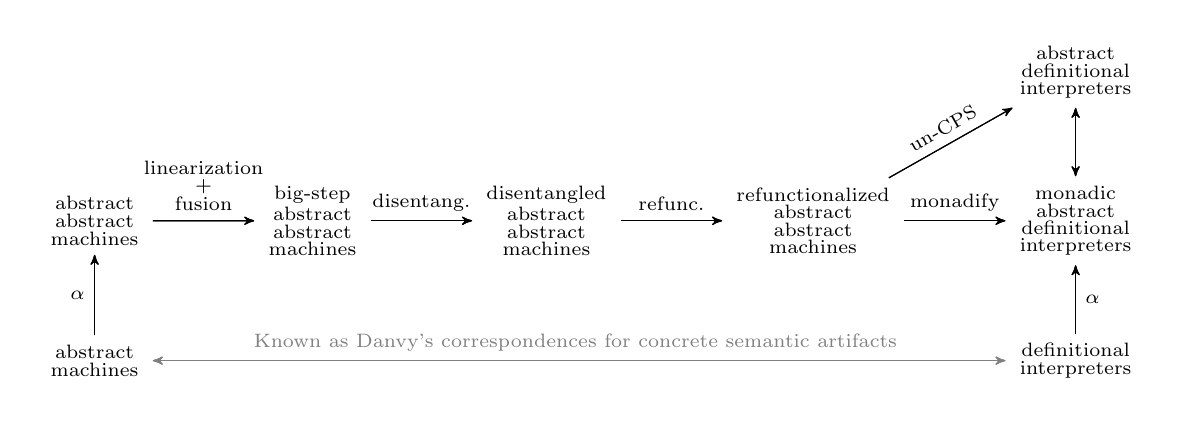
\begin{tikzpicture}
   \matrix (m) [matrix of math nodes, row sep=2.5em, column sep=3.7em]
     {
         &  &  &  &
       \begin{smallmatrix} \text{abstract} \\ \text{definitional} \\ \text{interpreters} \end{smallmatrix} \\
       \begin{smallmatrix} \text{abstract} \\ \text{abstract} \\ \text{machines} \end{smallmatrix} &
       \begin{smallmatrix} \text{big-step} \\ \text{abstract} \\ \text{abstract} \\ \text{machines} \end{smallmatrix}  &
       \begin{smallmatrix} \text{disentangled}  \\ \text{abstract} \\ \text{abstract} \\ \text{machines} \end{smallmatrix} &
       \begin{smallmatrix} \text{refunctionalized}  \\ \text{abstract} \\ \text{abstract} \\ \text{machines} \end{smallmatrix} &
       \begin{smallmatrix} \text{monadic} \\ \text{abstract} \\ \text{definitional} \\ \text{interpreters} \end{smallmatrix}  \\
       \begin{smallmatrix} \text{abstract} \\ \text{machines} \end{smallmatrix} &
         &
       %\begin{smallmatrix} \text{big-step} \\ \text{abstract} \\ \text{machines} \end{smallmatrix}  &
         &
       %\begin{smallmatrix} \text{disentangled} \\ \text{abstract} \\ \text{machines} \end{smallmatrix} &
         &
       %\begin{smallmatrix} \text{refunctionalized} \\ \text{abstract} \\ \text{machines} \end{smallmatrix} &
       \begin{smallmatrix} \text{definitional} \\ \text{interpreters} \end{smallmatrix} \\
     };
   {
     [start chain] \chainin (m-2-4);
     \chainin (m-1-5) [join={node[sloped,anchor=center,above,labeled] {\text{un-CPS}}}];
     \chainin (m-2-5) [join={node[above,labeled] {\text{}}}];
     \chainin (m-1-5) [join={node[above,labeled] {\text{}}}];
   }
   {
     [start chain] \chainin (m-2-1);
     \chainin (m-2-2) [join={node[above,labeled] {\begin{smallmatrix} \text{linearization} \\ \text{+} \\ \text{fusion} \end{smallmatrix}}     }];
     \chainin (m-2-3) [join={node[above,labeled] {\text{disentang.}}}];
     \chainin (m-2-4) [join={node[above,labeled] {\text{refunc.}}}];
     \chainin (m-2-5) [join={node[above,labeled] {\text{monadify}}}];
   }
   {
     [start chain]
     \chainin (m-3-1);
     { [start branch=A] \chainin (m-2-1)
       [join={node[left, labeled] {\alpha}}];
     }
   }
     %\chainin (m-2-2);
     %\chainin (m-2-3);
     %\chainin (m-2-4);
   {
     [start chain]
     \chainin (m-3-5);
     { [start branch=B] \chainin (m-2-5)
       [join={node[right, labeled] {\alpha}}];
     }
     {
       [start branch=D, color=gray] \chainin (m-3-1)
       [join={node[right, labeled] {\text{}}}];
     }
   }
   {
     [start chain, color=gray] \chainin (m-3-1);
     {
       [start branch=C] \chainin (m-3-5)
       [join={node[above, labeled] {\text{Known as Danvy's correspondences for concrete semantic artifacts }}}];
     }
   }
 \end{tikzpicture}
 \caption{Transformations from AAM to ADI} \label{fig:trans}
\end{center}
\end{figure}

\subsection{Contributions}

We begin by reviewing some background necessary for this work in Section~\ref{background}, 
as well as introducing some of the basic code structures used throughout the paper. 
We then address the main contribution of this paper, which is the filling of the gap between
small-step AAM and big-step ADI by applying a series of well-known systematic transformations
drawn from concrete semantic artifacts.
Figure \ref{fig:trans} shows the transformations.

Those transformations are summarized here, with their associated section:

\begin{itemize}
  \item We show \textbf{linearization} in Section~\ref{linear}. By expressing the
    nondeterministic choices as a first-order data type, we linearize the execution
    of abstract abstract machines; the transition of machine states therefore becomes 
    deterministic. Notably, this introduces another layer of control that will also 
    be refunctionalized later.

  \item In Section~\ref{fusing}, we then present the \textbf{lightweight fusion}.
    The fusing transformation simply combines the single-step function @step@ and the 
    driving function into one, but keeps all the machine state representations.

  \item Section~\ref{disen} discusses \textbf{disentanglement}, which disassembles the 
    fused AAM to be several individual functions, with each function handling one data 
    type representing continuation.

  \item \textbf{Refunctionalization} is shown in Section~\ref{sec:refunc} which sequentializes
    the order of abstract execution by higher-order functions. For clarity, we first present 
    the refunctionalized AAM without caching. We then adopt a different caching algorithm to 
    guarantee the termination of abstract interpretation.
    In this section, we also review pushdown control-flow analysis and examine how computable
    and precise call/return matching is obtained through these transformations.

  \item The last transformation we show is that of transforming the refunctionalized AAM to a
    \textbf{direct-style} interpreter (Section~\ref{directstyle}) by using delimited control operators.
\end{itemize}

These transformations are used throughout the paper, with refunctionalization and
defunctionalization of abstract interpreters playing important roles for the call stack of
the analyzed language. By refunctionalization, the call stack of the analyzed language
is blended into the call stack of the defining language. This provides another perspective to
explain why \citeauthor{darais2017abstracting}'s abstract definitional interpreters
is able to inherit the pushdown control-flow property from its defining language.

We complete this paper by discussing related work in Section~\ref{sec:related}, followed by 
concluding thoughts in Section~\ref{sec:conclusion}.

\iffalse
\subsection{Style}

We use Scala language to demonstrate the idea and each step of transformations.
We expect that readers have moderate familiarity to Scala's syntax, such as
case classes, pattern matching and for comprehension.

There are two main reasons we use a real-world language:
1) The code does not diminish the accuracy of the material than formal and mathematical
notations, which are heavily used in other static analysis or semantics papers.
The Scala code in this paper can be easily back-translated into formal notations.
2) As a functional pearl, the code in this paper is executable with only few changes,
which make it particularly fit for presenting syntactical transformations on abstract
interpreters.
\fi

\section{Background} \label{background}

\subsection{A-Normal Form $\lambda$-Calculus} \label{anfsyntax}

Traditionally, continuation-passing style (CPS) is a popular intermediate representation
for analyzing functional programs because it exposes control transfer explicitly and 
simplifies analysis~\cite{Shivers:1991:SSC:115865.115884, Shivers:1988:CFA:53990.54007}.
Here, we choose to use $\lambda$-calculus in administrative normal form (ANF)
\cite{flanagan1993essence}, which is a direct-style intermediate representation, as our 
target for clarity, but without losing simplicity and generality. The transformations 
we will show in the rest of this paper also work on abstract machines for plain 
direct-style $\lambda$-calculus languages. Although we only show the core calculus language,
it can be easily extended to support recursive bindings (such as @letrec@), conditionals, 
primitive types, and operations on primitive types. These cases would be straightforward to
implement without introducing new transformations as far as the concerns of this paper,
so we elide them here.
% TODO: appendix, direct-style, numbers and if0

To begin, we present the concrete syntax of a call-by-value $\lambda$-calculus language
in ANF.

%------------------------------------------------------------------------------------------------------------
\begin{lstlisting}
                                     x $\in$ Variables
                                    ae $\in$ AExp ::= ∂x | lam
                                   lam $\in$ Lam ∂::= (lambda (x) e)
                                     e $\in$ Exp ∂::= ae | (let ([x (ae ae)]) e)
\end{lstlisting}

In ANF, an expression is either an atomic expression or a @let@ expression.
A restriction exists which states that all function applications must be administrated
within a @let@ expression and then bound to a variable name under the current environment.
Both the operator and operand of function applications are atomic expressions.
An atomic expression $ae$ is either a variable or a literal @lambda@ term, either of which
can be evaluated in a single step. We also assume that all the variable names in the program
 are unique.

The abstract syntax in Scala is shown as follows. We assume that the source program conforms
to the ANF convention, and we do not enforce it in the term structure of Scala constructs.

\begin{lstlisting}
  sealed trait Expr
  case class Var(x: String) extends Expr
  case class App(e1: Expr, e2: Expr) extends Expr
  case class Lam(x: String, body: Expr) extends Expr
  case class Let(x: String, e: App, body: Expr) extends Expr
\end{lstlisting}

\subsection{CESK Machine} \label{cesk}

\subsubsection{Machine Components}

The CESK machine is an abstract machine for describing semantics of and evaluating 
$\lambda$-calculus \cite{felleisen1987calculus}. The CESK machine models program execution 
as state transitions in a small-step fashion. As its name suggests, a machine state has 
four components:
1) \textit{Control} is the expression currently being evaluated.
2) \textit{Environment} is a map that contains the address of a variable in the lexical scope.
3) \textit{Store} models the heap of a program as a map from addresses to values.
  The address space consists of numbers (0-indexed).
  In our toy language, the only category of value is a closure, i.e., a function paired with
  an environment.
4) \textit{Continuation} represents the program's call stack. In this paper, we instantiate the 
  stack as a list of frames because the ANF simplifies the evaluation context. For direct % TODO
  style $\lambda$-calculus, the continuations of CEK/CESK machines can be presented by
  variants of a data type.

The Scala representations for the components of the CESK machine are as follows:

\begin{lstlisting}
  type Addr = Int;     type Env = Map[String, Addr];    type Store = Map[Addr, Storable]
  abstract class Storable
  case class Clos(v: Lam, env: Env) extends Storable
  case class Frame(x: String, e: Expr, env: Env);       type Kont = List[Frame]
  case class State(e: Expr, env: Env, store: Store, k: Kont)
\end{lstlisting}

It is worth noting that the continuation class @Kont@ is defined as a list of
frames, where a frame can be considered a reduction context in reduction semantics.
We represent frames using the @Frame@ class, which stores the information of a single
call-site, i.e., the information that can be used to resume the interrupted computation.
A @Frame@ constitutes a variable name @x@ to be bound later, and a control component
to which the program may resume, and its environment.

\subsubsection{Single-Step Transition}
Before describing how the machine evaluates expressions, we must first define several helper
functions. As mentioned in Section~\ref{anfsyntax}, atomic expressions are either a variable
or a literal @lambda@ term. As such, the atomic expression evaluator @atomicEval@ handles
these two cases and evaluates atomic expressions to closures in a straightforward way.
The @alloc@ function generates a fresh address, and always allocates a unique integer
in the domain of @store@.
The @isAtomic@ function is used as a predicate to determine if the expression is atomic.

\begin{lstlisting}
  def atomicEval(e: Expr, env: Env, store: Store): Storable = e match {
    case Var(x) => store(env(x))
    case lam @ Lam(x, body) => Clos(lam, env)
  }
  def alloc(store: Store): Addr = store.keys.size + 1
  def isAtomic(e: Expr): Boolean = e.isInstanceOf[Var] || e.isInstanceOf[Lam]
\end{lstlisting}

We can now faithfully describe the state transition function @step@,
which when given a machine state, determines its successor state.
The function @step@ is a partial function that only handles non-final states,
which must have a successor; the final case of a state is handled by funciton
@drive@, which will be mentioned in the next section.

\begin{lstlisting}
  def step(s: State): State = s match {
    case State(Let(x, App(f, ae), e), env, store, k) if isAtomic(ae) =>
      val Clos(Lam(v, body), env_c) = atomicEval(f, env, store)
      val addr = alloc(store)
      val new_env = env_c + (v -> addr)
      val new_store = store + (addr -> atomicEval(ae, env, store))
      val frame = Frame(x, e, env)
      State(body, new_env, new_store, frame::k)
    case State(ae, env, store, k) if isAtomic(ae) =>
      val Frame(x, e, env_k)::ks = k
      val addr = alloc(store)
      val new_env = env_k + (x -> addr)
      val new_store = store + (addr -> atomicEval(ae, env, store))
      State(e, new_env, new_store, ks)
  }
\end{lstlisting}

As shown and previously discussed, we examine the only two non-final cases which the state
may be.

\begin{itemize}

\item In the first @case@ statement shown in the previous code, the control of the current 
  state matches as a @Let@ expression, with its right-hand side a function application.
  By calling the @atomicEval@ evaluator, we obtain the closure for which the callee @f@ stands.
  The successor state's control then transfers to the @body@ expression of the closure with 
  an updated environment and store. The new environment is extended from the closure's 
  environment and mapped from @v@ to a fresh address @addr@. The new store is extended with
  @addr@ mapping to the value of @ae@, which in turn is evaluated from @atomicEval@.
  Finally, a new frame @frame@ is pushed onto the stack @k@, where the @frame@ contains 
  the variable name @x@ at the left-hand position of the @Let@, the body expression of 
  @Let@, and the lexical environment of the body expression.

\item If the control component is not a @Let@ expression, then it must be an atomic
  expression, as seen in the above code. In this scenario, we begin by extracting the
  top frame of all available continuations. The variable @x@ from the top frame will
  be bound to the result of evaluating the atomic expression @ae@ by updating the
  environment and store.
  Finally, the successor state is transferred to expression @e@ from the top frame,
  which is the body of a @Let@ expression, with the updated environment, store, and
  the rest of the stack @ks@.

\end{itemize}

\subsubsection{Valuation}

To run the program, we first use the @inject@ function (below) to construct an initial 
machine state given a closed expression @e@. The initial state contains an empty environment,
store, and stack.
\begin{lstlisting}
  def inject(e: Expr): State = State(e, Map(), Map(), Nil)
\end{lstlisting}

The @drive@ function is then used to evaluate to a final state by iteratively applying 
@step@ on the current state until a state is reached which the control is an atomic 
expression and the continuation stack is empty. Naturally, we can then extract the value
from the final state at last.

\begin{lstlisting}
  def drive(s: State): State = s match {
    case State(ae, _, _, Nil) if isAtomic(ae) => s
    case _ => drive(step(s))
  }
  def eval(e: Expr): State = drive(inject(e))
\end{lstlisting}

\subsection{Abstracting Abstract Machines} \label{aam}
Abstracting abstract machines (AAM) is a systematic methodology that derives sound
abstract interpreters for higher-order functional languages from concrete abstract 
machines \cite{van2012systematic, van2010abstracting}. An abstracting abstract machine
implements computable abstract semantics which approximates the runtime behaviors of 
programs.
Since the state space of concrete execution is possibly infinite, the key insight of 
AAM approach when analyzing programs is to allocate both bindings and continuations 
on the store, and then bound the addresses space to be finite. Since each component
of state is finite, the abstracted machine-state space is also finite, and therefore
computable.

In this section, we derive the abstracting abstract machine from concrete
CESK machines, and also show how to instantiate useful $k$-call-sensitive 
control-flow analysis.

\subsubsection{Machine Components}

Similar to CESK machines, the machine state of AAM has a control, an environment, a store,
and continuation, as well as a timestamp. However, there are several notable differences
between AAM's store and CESK machine's store. In AAM, the store maps addresses to sets of
values; it stores all possible values for a particular address. As such, dereferencing
addresses becomes nondeterministic. Also, the store performs \emph{joining}, rather than
overwriting, when updating elements. Furthermore, the continuations are likewise allocated
on the store instead of formed into a linked list, and the continuation component becomes
an address that maps to a set of continuations in the store instead of directly embedded
in the state.

For clarity, we divide the store into two separate stores: the binding stores @BStore@, and
the continuation store @KStore@.
The binding store maps binding addresses to sets of closure values, whereas the continuation
store maps continuation addresses to sets of continuations.
We then define a generic class @Store[K,V]@ that performs joining when updating elements
in a store (below). By parameterizing @Store[K,V]@ with @[BAddr, Storable]@ and
@[KAddr, Cont]@, we obtain @BStore@ and @KStore@, respectively.
We note that both the value store and continuation store are uodated monotonically;
it continuously grows and never shrinks.

\begin{lstlisting}
  case class Store[K,V](map: Map[K, Set[V]]) {
    def apply(addr: K): Set[V] = map(addr)
    def update(addr: K, d: Set[V]): Store[K,V] = {
      val oldd = map.getOrElse(addr, Set())
      Store[K, V](map ++ Map(addr -> (d ++ oldd)))
    }
    def update(addr: K, sd: V): Store[K,V] = update(addr, Set(sd))
  }
  type BStore = Store[BAddr, Storable];  type KStore = Store[KAddr, Cont]
\end{lstlisting}

The codomain of binding stores @Storable@ is the same as previously defined for CESK 
machines. The codomain of continuation stores @Cont@, on the other hand, is comprised of
a @Frame@ object and a continuation address @KAddr@. To mimic the runtime call stack, 
@KAddr@ plays the role of representing the remaining stack frames.
But since the continuation store may contain multiple continuations, the dereferencing 
of continuation addresses is also nondeterministic.

\begin{lstlisting}
  case class Frame(x: String, e: Expr, env: Env);      case class Cont(frame: Frame, kaddr: KAddr)
\end{lstlisting}

As a consequence, the components of states are also changed: the store is divided
into binding stores and continuation stores; the continuation becomes an address
that maps to a set of continuations in @KStore@.
By dereferencing this address in a continuation store, we can retrieve the actual 
transfers of control. The definition of environment @Env@ remains the same.

\begin{lstlisting}
  case class State(e: Expr, env: Env, bstore: BStore, kstore: KStore, k: KAddr, time: Time)
\end{lstlisting}

\subsubsection{Allocating Addresses}
Up to this point, we have not described allocating addresses in stores, nor handling
the time stamp @Time@. In abstract interpretation, however, these are key ingredients
to achieve analyses with different sensitivities, as well as to perform a finite
state space analysis \cite{Gilray:2016:ACP:2951913.2951936}.
To effectively approximate the runtime behavior, we introduce a finite program contours
@time@ that encodes the program execution history. The function @tick@ is used to refresh
the "time" and get a "new time". We use a list of expression (which are drawn from the
control component) to encode the calling contexts history, and as we will see in Section~
\ref{kcfainst}, by applying different @tick@ functions on the timestamp, we are able to
obtain a family of analyses.

\begin{lstlisting}
  type Time = List[Expr]
\end{lstlisting}

As previously mentioned, the space of states is finite when the space of addresses is finite.
To make this happen, binding addresses are parameterized by variable names and the creation
time of the binding, both of which are finite. Continuation addresses @KAddr@ has two variants:
1) @Halt@ which corresponds to the empty stack, and
2) @ContAddr@ consists of the target expressions of callee, which are also finite.
%One may ask, why not also keep track of the time in continuation addresses?
%\todo{why target expression, allocation polyvariance}

\begin{lstlisting}
  case class BAddr(x: String, time: Time) 
  abstract class KAddr
  case object Halt extends KAddr
  case class ContAddr(tgt: Expr) extends KAddr
\end{lstlisting}

We introduce two helper functions, @allocBind@ and @allocKont@, which will be
used to allocate binding addresses and continuation addresses.

\begin{lstlisting}
  def allocKont(tgtExpr: Expr): KAddr = ContAddr(tgtExpr)
  def allocBind(x: String, time: Time): BAddr = BAddr(x, time)
\end{lstlisting}

Given that the space of addresses is finite, we can conclude that there are finite number
of environments and stores because the numbers of variables and closures are also finite.
This property guarantees a finite space of reachable states, and we can always have a
terminated analysis through Kleene's fixed-point iteration.

\subsubsection{Single-Step Transition}

Since dereferencing an address becomes nondeterministic, our @atomicEval@
function (below) is also nondeterministic. Given an atomic expression @e@,
@atomicEval@ returns a set of storable values (i.e., closures) to the caller.
If the expression is simply a @lambda@ term, the returned set is a singleton.

\begin{lstlisting}
  def atomicEval(e: Expr, env: Env, bstore: BStore): Set[Storable] = e match {
    case Var(x) => bstore(env(x))
    case lam@Lam(x, body) => Set(Clos(lam, env))
  }
\end{lstlisting}

The structure of function @step@ is similar to the concrete CESK machine,
except the nondeterminism which makes @step@ return a list of reachable successor states.
We have two cases to consider (code shown below):

\begin{itemize}
  \item If the current control component is a @Let@, then the result of @App(f, ae)@ will 
    be bound to variable @x@. In this case, we retrieve the set of closures that @f@ may 
    represent. For each closure in the set, we perform nearly the same operations as in the
    concrete CESK machines, with an important difference: the continuation is allocated on 
    the store @kstore@, so a new continuation address @new_kaddr@ must be constructed and 
    a new frame @Frame(x, e, env)@ paired with the current continuation address @kaddr@ is 
    merged into @new_kaddr@. Finally, a list of successor states is generated.

  \item In the second case, an atomic expression @ae@ sits on the control position of the
    state. Here, the value of @ae@ is being returned to its caller.
    In order to accomplish this, we dereference the continuation address @kaddr@ and obtain 
    a set of continuations @conts@. For each continuation in the set, we construct an 
    environment based on the environment @env_f@ of the frame, and bind @x@ to a newly 
    created binding address @baddr@. We must also update the store with @baddr@ and the 
    values that @ae@ represents. In every generated state, the control becomes the expression 
    @e@ in the frame, and as we can tell from the name, the continuation address @f_kaddr@ 
    also comes from the frame.
\end{itemize}

\begin{lstlisting}
  def step(s: State): List[State] = {
    val new_time = s.tick
    s match {
      case State(Let(x, App(f, ae), e), env, bstore, kstore, kaddr, time) =>
        val closures = atomicEval(f, env, bstore).toList
        for (Clos(Lam(v, body), env_c) <- closures) yield {
          val baddr = allocBind(v, new_time)
          val new_env = env_c + (v -> baddr)
          val new_bstore = bstore.update(baddr, atomicEval(ae, env, bstore))
          val new_kaddr = allocKont(body)
          val new_kstore = kstore.update(new_kaddr, Cont(Frame(x, e, env), kaddr))
          State(body, new_env, new_bstore, new_kstore, new_kaddr, new_time)
        }
      case State(ae, env, bstore, kstore, kaddr, time) if isAtomic(ae) =>
        val conts = kstore(kaddr).toList
        for (Cont(Frame(x, e, env_f), f_kaddr) <- conts) yield {
          val baddr = allocBind(x, new_time)
          val new_env = env_f + (x -> baddr)
          val new_store = bstore.update(baddr, atomicEval(ae, env, bstore))
          State(e, new_env, new_store, kstore, f_kaddr, new_time)
        }
    }
  }
\end{lstlisting}

\subsubsection{$k$-Call-Sensitive Instantiation} \label{kcfainst}

In $k$-call-sensitive analysis, a history of the last $k$ call sites is used as a 
finite program contour. The history is represented as a list of expressions and embedded
in the allocated addresses.

Before transferring to successor states, we must use the @tick@ function to refresh the 
timestamp, and then use this new timestamp for successors when allocating addresses.
The @tick@ function returns the $k$ front-most expressions given the current state and its
time history. We implement @tick@ as a public method of case class @State@.

\begin{lstlisting}
  def k: Int = 0
  case class State(e: Expr, env: Env, bstore: BStore, kstore: KStore, kaddr: KAddr, time: Time) {
    def tick: Time = (e :: time).take(k)
  }
\end{lstlisting}

If we instantiate $k$ to be $0$, the history degenerates to an empty list, and we obtain
a monovariant analysis (i.e., it does not differentiate values at different call sites).
In this case, the address space collapses to the space of variable names.
Note that regarding the ambiguity in $k$-CFA\cite{Gilray:2016:ACP:2951913.2951936},
the code here actually implements call+return sensitivity.

\subsubsection{Collecting Semantics}

Similar to the CESK machines, to run (analyze) a program we first use the @inject@ function
to construct the initial state given to the program. Note that the initial continuation store
has a built-in mapping that maps the continuation address for @Halt@ to an empty set of 
continuations. We also provide an empty program contour as our initial time.

\begin{lstlisting}
  val mtTime = List();                         val mtStore = Store[BAddr, Storable](Map())
  val mtEnv = Map[String, BAddr]();            val mtKStore = Store[KAddr, Cont](Map(Halt -> Set()))
  def inject(e: Expr): State = State(e, mtEnv, mtStore, mtKStore, Halt, mtTime)
\end{lstlisting}

However, in contrast to the concrete CESK machine, the @drive@ function performs 
collecting semantics instead of the valuation semantics. That is, for the purpose of
analyzing programs, the function @drive@ collects all the intermediate machine states 
as the program is abstractly executing. The following code shows a variant of the 
worklist algorithm to find the fixed-point of the set of states.
Function @drive@ always applies function @step@ to the head element @hd@ of
the worklist @todo@ if @hd@ is unseen. It then inserts the result of @step@ to
the rest of worklist, and in the meantime adds @hd@ to the explored states set.
If the worklist is empty, @drive@ simply returns the set of reachable states
up to the current execution point.

\begin{lstlisting}
  def drive(todo: List[State], seen: Set[State]): Set[State] = todo match {
    case Nil => seen
    case hd::tl if seen.contains(hd) => drive(tl, seen)
    case hd::tl => drive(step(hd).toList ++ tl, seen + hd)
  }
  def analyze(e: Expr): Set[State] = drive(List(inject(e)), Set())
\end{lstlisting}

Finally, a user may invoke the @analyze@ function to obtain all reachable states for 
a given program.

%\subsection{Monadic Abstract Interpreter}
%Maybe not here?

\subsection{One Step Back: Unabstracted Stack} \label{unabs}

In this section, we describe a variant of AAM that allows the stack to be
unbounded which uses a precise call stack as we did in the concrete CESK machine.
Instead of allocating continuations in the store and embedding addresses of 
continuations in states, we intend to use a list of frames to explicitly model 
the stack. By doing so, we recover the call stack as the same as runtimes
(so called pushdown control-flow analysis), but since the stack is unbounded, 
the state space is potentially infinite. 

The pushdown AAM with unbounded stack is also described by \citeauthor{van2012systematic} 
\cite{van2012systematic}. 
The reason we show it here is to keep the consistency of abstract semantics during 
transformations -- since the eventual abstract definitional interpreters simply inherit
a precise control-flow from its defining language, we also would like to start from a
pushdown AAM that is also able to precisely match calls and returns.
For readers who are not familiar with pushdown analysis, we have a detailed discussion 
in Section~\ref{pdcfarevisit}.

In the definition of @State@, the continuation store and continuation address disappear;
instead, a list of frames represents the stack. An empty list denotes that we have reached 
the halt. The other components remain unchanged as in the Section \ref{aam}.

\begin{lstlisting}
  case class State(e: Expr, env: Env, bstore: BStore, konts: List[Frame], time: Time)
\end{lstlisting}

The state transition function @step@ shown below is still nondeterministic, but the only 
nondeterminism happening is when dereferencing the callee @f@ from the function application 
@App(f, ae)@.

\begin{lstlisting}
  def step(s: State): List[State] = {
    val new_time = s.tick
    s match {
      case State(Let(x, App(f, ae), e), env, bstore, konts, time) if isAtomic(ae) =>
        for (Clos(Lam(v, body), env_c) <- atomicEval(f, env, bstore).toList) yield {
          val frame = Frame(x, e, env)
          val baddr = allocBind(v, new_time)
          val new_env = env_c + (v -> baddr)
          val new_store = bstore.update(baddr, atomicEval(ae, env, bstore))
          State(body, new_env, new_store, frame::konts, new_time)
        }
      case State(ae, env, bstore, konts, time) if isAtomic(ae) =>
        konts match {
          case Nil => List()
          case Frame(x, e, env_f)::konts =>
            val baddr = allocBind(x, new_time)
            val new_env = env_f + (x -> baddr)
            val new_store = bstore.update(baddr, atomicEval(ae, env, bstore))
            List(State(e, new_env, new_store, konts, new_time))
        }
    }
  }
\end{lstlisting}

In the first case of pattern matching, we may have multiple choices of closure for callee @f@.
For each closure in the set, a new frame is constructed and pushed onto the stack.
The code for handling the second case (atomic expressions) is the same as the concrete CESK machines. \\

\textit{Note on Termination.}
Unfortunately, even though other components in the states are finite, this AAM with an unbounded
stack still may diverge when analyzing some programs.
This is because the unbounded stack can grow to arbitrary depth which implies that the state
space is possibly infinite; the analysis may therefore not terminate for all programs if we
simply enumerate reachable states. To see this, consider a program that has two mutually
recursive functions:

\begin{lstlisting}
                                  (letrec ([f1 (lambda (x)
                                                 (let ([x1 (f2 x)]) x1))]
                                           [f2 (lambda (y)
                                                 (let ([y1 (f1 y)]) y1))])
                                    (let ([z (f1 1)])
                                      z))
\end{lstlisting}

Function @f1@ and @f2@ mutually invoke each other, so the stack will alternately pushing
frames @f1@ and @f2@ onto the top of current stack. However, no two existing stack
components are identical in the state space. One can decide the reachability of a state
through Dyck state graph \cite{earl2010pushdown, earl2012introspective}, but simply
caching the explored states (i.e. @seen@) would not always make the analyzer terminate.


\section{Linearization} \label{linear}

In the previous section, we show that by keeping an unabstracted stack in the state
space, we can recover the precise call/return match. Now we begin describing the
transformations step by step. Our base machine for now is the AAM with unbounded
stack, though as we will later transform the stack to higher-order functions
representing continuations, it does not matter what kind of AAM we start from.
This is because transforming to higher-order functions forces us to sequentialize
the order of abstract evaluation, and neither requiring construction of a frame on
stack, nor to allocate continuations in the store.
Thus, our choice to start from an AAM with unbounded stack is motivated simply because
it has an equivalent stack model to abstract definitional interpreters (our final target).

The underlying semantics of AAM is fundamentally nondeterministic: there are possibly
multiple target closures when dereferencing an address, and we have to explore both branches
if the conditionals exist in the language. But the reduction context (i.e., the @Frame@ in
our program) is \emph{not} nondeterministic, and the worklist @todo@ actually implicitly
handles the nondeterminism. Thus, if we simply refunctionalize the frames to higher-order
functions, it does not help us to move toward abstract definitional interpreters.

In Danvy's paper \textit{Defunctionalized Interpreters for Programming Languages},
he mentions that for deterministic languages, a reduction semantics is a structural
operational semantics in continuation-passing style, where the reduction context is
a defunctionalized continuation \cite{Danvy:2008:DIP:1411204.1411206}. Therefore
refunctionalizing a deterministic language yields an interpreter in continuation-passing
style; nevertheless, doing so for nondeterministic languages yields an interpreter
with multiple layers of continuation \cite{Danvy:2006:RW:2171265.2171268}.

We apply this idea to AAM and our first step of transformations is to linearize all
nondeterministic choices. This step removes all nondeterminism from the @step@ function.
Likewise, the @Frame@ saves the information of the caller in concrete executions.
We then introduce another layer of control, and define a case class @NDCont@
that saves the information at a fork point when we have multiple target closures.
We also add a new field @ndk@ to the definition of state, which we now call @NDState@.
For clarity of presentation in differentiating between the two continuations, we elect to call
the first a \emph{normal continuation}, and the second a \emph{meta-continuation}
\footnote{Traditionally, they are also called \emph{success continuation} and \emph{failure
continuation} \cite{Danvy:1990:AC:91556.91622}.}.

\begin{lstlisting}
  case class NDCont(cls: List[Clos], argvs: Set[Storable], store: BStore, time: Time, frames: List[Frame])
  case class NDState(e: Expr, env: Env, bstore: BStore, konts: List[Frame], time: Time, ndk: List[NDCont]) {
    def toState: State = State(e, env, bstore, konts, time)
    def tick: Time = ...
  }
\end{lstlisting}

Here we also use first-order data types to explicitly represent the meta-continuation which
controls the nondeterminism.
Each @NDCont@ object contains a list of closures that are possible functions to be invoked,
a set of values that will be bound to the function's formal argument, and the store, time,
and frames at the fork point. In the definition of @NDState@, an auxiliary function @toState@
is added that converts itself to @State@.

Function @step@ now becomes of type @NDState => NDState@.
The following code shows the first case of matching an instance of @NDState@ in
the @step@ function:

\begin{lstlisting}
  case NDState(Let(x, App(f, ae), e), env, bstore, konts, time, ndk) =>
    val closures = atomicEval(f, env, bstore).toList.asInstanceOf[List[Clos]]
    val Clos(Lam(v, body), c_env) = closures.head
    val frame = Frame(x, e, env)
    val new_frames = frame::konts
    val baddr = allocBind(v, new_time)
    val new_env = c_env + (v -> baddr)
    val argvs = atomicEval(ae, env, bstore)
    val new_store = bstore.update(baddr, argvs)
    val new_ndk = NDCont(closures.tail, argvs, bstore, new_time, new_frames)::ndk
    NDState(body, new_env, new_store, new_frames, new_time, new_ndk)
\end{lstlisting}

By atomically evaluating @f@, we obtain a set of closures, with the transition being 
deterministic in regards to the first element of the closure set.
As such, we prepare a new environment, a new store, and a new frame list only for the
first closure in that set. A new meta-continuation @new_ndk@ is also constructed,
which contains the rest of closures, the values of argument @ae@, the store, the time,
and the new frame list. We use the store before updating, because for different closures
they may form different binding addresses @baddr@. We also use the new frames, because
all closures at this fork point share the same stack and return point.

In the second case (shown below), we will see how @NDCont@ deals with nondeterminism.

\begin{lstlisting}
  case NDState(ae, env, bstore, konts, time, ndk) if isAtomic(ae) =>
    konts match {
      case Nil => ndk match {
        case NDCont(Nil, _, _, _, _)::ndk =>
          NDState(ae, env, bstore, konts, time, ndk) /* transfer to the most recent fork point */
        case NDCont(cls, argvs, bstore, time, frames)::ndk =>
          val Clos(Lam(v, body), c_env) = cls.head
          val baddr = allocBind(v, time); val new_env = c_env + (v -> baddr)
          val new_store = bstore.update(baddr, argvs)
          val new_ndk = NDCont(cls.tail, argvs, bstore, tile, frames)::ndk
          /* resume the fork point with the next closure */
          NDState(body, new_env, new_store, frames, time, new_ndk)
      }
      case Frame(x, e, f_env)::konts =>
        val baddr = allocBind(x, newTime); val new_env = f_env + (x -> baddr)
        val new_store = bstore.update(baddr, atomicEval(ae, env, bstore))
        NDState(e, new_env, new_store, konts, newTime, ndk) /* normal return */
    }
\end{lstlisting}

If the normal continuation @konts@ is an empty list, then it means we have reached
the end of the computation (i.e., a halt); otherwise, we should return the values of 
@ae@ to its caller which is contained in the top frame of stack.

However, since we have added nondeterminism into state, an empty list of frames means
we have reached the halt of \textit{one computation path}, and we should determine the
next state indicated by @NDCont@. Thus, we have a pattern matching on @ndk@:

\begin{itemize}
  \item If the closure set is an empty set,
then we have tried all the closures of this fork point and should move to the
next fork point. Since the @NDCont@ is represented by a list, and we always
append new elements to its front, we are resuming to the most recent fork point by
popping up the front-most element.
  \item Otherwise, we pop a closure from the set, then build a new
environment and a new store for the body expression of the closure;
we use the same frame list and time that are copied from the fork point rather
than current one.
The meta-continuation @new_ndk@ is also updated by the removal of that closure.
\end{itemize}

\begin{lstlisting}
  def drive(nds: NDState, seen: Set[State]): Set[State] = {
    nds match {
      case NDState(ae, _, _, Nil, _, Nil) if isAtomic(ae) => seen
      case nds =>
        val s = nds.toState
        if (seen.contains(s)) drive(step(nds), seen)
        else drive(step(nds), seen + s)
    }
  }
\end{lstlisting}

The @drive@ function is also changed: there is no worklist anymore, as all the
potentially unexplored states are embedded into the continuation for
nondeterminism.
The termination of the analysis occurs when we reach an @NDState@ in which the expression
is atomic and both the normal continuation and nondeterminism continuation are
empty lists. This corresponds to the case that @todo@ list is empty.

At this point, we have obtained a linearized abstract abstract machine. If we imagine that the
classical AAM explores a graph of reachable states, then the linearized AAM flattens the
graph to a linear sequence.

\section{Lightweight Fusion} \label{fusing}

Then we apply a lightweight fusion transformation that combines the @step@ and @drive@
functions into a single function.
The fused function @drive_step@ is essentially formed by merging the functionality of
@step@ into the @drive@ function.
@drive_step@ takes an @NDState@ and a set of explored states as an argument
and returns a set of reachable states once it terminates.

\begin{lstlisting}
  def drive_step(nds: NDState, seen: Set[State]): Set[State] = {
    nds match {
      case NDState(ae, _, _, Nil, _, Nil) if isAtomic(ae) => seen
      case nds =>
        val s = nds.toState; val newTime = nds.tick
        val new_seen = if (seen.contains(s)) seen else seen+s
        val new_ndstate = nds match {
          case NDState(Let(x, App(f, ae), e), env, bstore, konts, time, ndkonts) => ...
          case NDState(ae, env, bstore, konts, time, ndkonts) if isAtomic(ae) => ...
        }
        drive_step(new_ndstate, new_seen)
    }
  }
\end{lstlisting}

With this, we have a single function to perform both abstract evaluation and the collection of
intermediate states. Given @inject(e)@ as an initial state and an empty set as the
initial set of states reached, we can easily define the entrance function @analyze@ as
follows:

\begin{lstlisting}
  def analyze(e: Expr): Set[State] = drive_step(inject(e), Set())
\end{lstlisting}

\section{Disentanglement} \label{disen}

With fusing complete, our AAM appears similar to a ``big-step'' interpreter, although it
still has the machine state representation inside. In the disentanglement transformation,
we identify the first-order data types which represent reduction contexts
and lift the code blocks that handle these reduction contexts to be individual functions.

Since there are two layers of continuations, we obtain three mutually recursive functions:
@drive_step@, which plays the same role as before; @continue@, which is called from
@drive_step@ when encountering an atomic expression, and handles the reduction context
(@Frame@) of the analyzed language; and @ndcontinue@, which dispatches meta-continuations
@NDCont@, and which is invoked from @continue@ when the normal stack is empty.

\begin{lstlisting}
  def drive_step(nds: NDState, seen: Set[State]): Set[State] = {
    nds match {
      case NDState(ae, _, _, Nil, _, Nil) if isAtomic(ae) => seen
      case nds =>
        val s = nds.toState; val new_time = nds.tick
        val new_seen = if (seen.contains(s)) seen else seen + s
        nds match {
          case NDState(Let(x, App(f, ae), e), env, bstore, konts, time, ndk) =>
            ...
            drive_step(NDState(body, new_env, new_store, new_frames, new_time, new_ndk), new_seen)
          case NDState(ae, env, bstore, konts, time, ndk) if isAtomic(ae) =>
            continue(nds, new_seen)
        }
    }
  }
\end{lstlisting}

The above code shows the skeleton of @drive_step@.
At the end of the first case of pattern matching, we invoke @drive_step@ recursively 
\footnote{The code for constructing new environments, stores, and frames is elided for 
simplicity of presentation.}.
The code for the second case is replaced entirely by a function call to @continue@.
The shape of an interpreter in continuation-passing style has emerged.

\begin{lstlisting}
  def continue(nds: NDState, seen: Set[State]): Set[State] = {
    val NDState(ae, env, bstore, konts, time, ndk) = nds; val new_time = nds.tick
    konts match {
      case Nil => ndcontinue(nds, seen)
      case Frame(x, e, f_env)::konts =>
        val baddr = allocBind(x, new_time); val new_env = f_env + (x -> baddr)
        val new_store = bstore.update(baddr, atomicEval(ae, env, bstore))
        drive_step(NDState(e, new_env, new_store, konts, new_time, ndk), seen)
    }
  }
\end{lstlisting}

Function @continue@ is mainly what we have seen for the second case in @drive_step@,
except that @ndcontinue@ is called when the normal continuation is empty.
Since we are analyzing a language in ANF, the first-order data representation of
continuations is simplified to a Scala @List@. An empty list @Nil@ represents the %TODO
halt of a computation path, whereas a cons @::@ means the top frame of the list
holds the binding variable and context.
An analogy to this in standard CEK machines would be an abstract class (e.g., @cont@)
with three variants: @halt@, @arg(value, cont)@, and @arg(exp, env, cont)@.

\begin{lstlisting}
  def ndcontinue(nds: NDState, seen: Set[State]): Set[State] = {
    val NDState(ae, env, bstore, konts, time, ndk) = nds
    ndk match {
      case NDCont(Nil, _, _, _, _)::ndk =>
        drive_step(NDState(ae, env, bstore, konts, time, ndk), seen)
      case NDCont(cls, argvs, bstore, time, frames)::ndk =>
        val Clos(Lam(v, body), c_env) = cls.head
        val baddr = allocBind(v, time); val new_env = c_env + (v -> baddr)
        val new_store = bstore.update(baddr, argvs)
        val new_ndk = NDCont(cls.tail, argvs, bstore, time, frames)::ndk
        drive_step(NDState(body, new_env, new_store, frames, time, new_ndk, seen))
    }
  }
\end{lstlisting}

The shape for @ndcontinue@ is similar to @continue@; after
all, they both use a @List@ representation for continuations.
When the closure set is empty, we recursively call @drive_step@ with the rest
of @ndk@, since in this case the normal stack @konts@ is still empty, so
the state will be dispatched to @ndcontinue@ again.
Otherwise, we invoke @drive_step@ with the body expression of the next closure object.

\section{Refunctionalization} \label{sec:refunc}

Refunctionalization transforms first-order data types representing
evaluation contexts to higher-order functions.
Besides sequentializing the order of abstract evaluation by functions,
this transformation can be also regarded as allocating continuation functions of
the defined language in the heap of the metalanguage.

In this section, several other notable changes have been made:
\begin{itemize}
\item We do not have the concept of @state@ (or @NDState@) anymore.
The components of the states are lifted as arguments of the evaluation
function.
\item Since our final target is an abstract definitional interpreter (though still
nondeterministic), starting from this section our abstract semantic artifact
returns a set of final values instead of collected states.
\item As we are getting close to achieving
abstract definitional interpreters, the name of @drive_step@ is updated to
@aeval@ (for \emph{abstract eval}).
\end{itemize}

For clarity, we first show how to refunctionalize normal continuations and
meta-continuation without collecting semantics.
Then, adding an appropriate caching algorithm to make sure the analysis will
terminate at some fixed-point is a simple transformation of the program to cache-passing
style. Finally, we examine how computable pushdown control-flow analysis is established
through refunctionalization and caching.

\subsection{First Try}

To properly represent final values, we introduce the case class @VS@ which
contains a set of storable values, a timestamp, and a store.

\begin{lstlisting}
  case class VS(vals: Set[Storable], time: Time, store: BStore)
\end{lstlisting}

An instance of @VS@ represents the computational result of one path in
the nondeterministic evaluation.
The reason that we include a store is that there might be a case in which two paths
have the same values but different accumulated side effects (e.g., memory allocations).
Since the whole computation is potentially nondeterministic, the type of the final result
values is a collection @Set[VS]@. For convenience, we define it as a type @Ans@:

\begin{lstlisting}
  type Ans = Set[VS]
\end{lstlisting}

As previously mentioned, the components of states are lifted as arguments to
@aeval@. Therefore, the pattern matching on the state becomes just a match on
expression @e@. The shape of function @aeval@ looks like:

\begin{lstlisting}
  type Cont = Ans => Ans
  def aeval(e: Expr, env: Env, store: BStore, time: Time, continue: Cont): Ans = {
    val new_time = ...
    e match {
      case Let(x, App(f, ae), e) => ...
      case ae if isAtomic(ae) => ...
    }
  }
\end{lstlisting}

An additional argument @continue@ which has type @Cont@ is also introduced.
Recall that in the disentangled AAM, the second case in @drive_step@
makes a call to @continue@. Here, the reemerging @continue@ is a function
of type @Ans => Ans@. The function @aeval@ does not return: instead, it calls
@continue@ with the result values. \\

\textit{Nondeterminism Abstractions.}
To handle the inevitable nondeterminism, we define a generic function @nd@ as follows:

\begin{lstlisting}
  def nd[T](ts: Iterable[T], acc: Ans, k: (T, Ans => Ans) => Ans, m: Ans => Ans): Ans = {
    if (ts.isEmpty) m(acc)
    else k(ts.head, (ans: Ans) => nd(ts.tail, acc ++ ans, k, m))
  }
\end{lstlisting}

Given a collection of elements of type @T@, an initial accumlator of type 
@Ans@, a function @k@ that works on element's type @T@ and takes a continuation 
of type @Ans=>Ans@, and a function @m@ that works on and returns a value of type 
@Ans@ (which is also type @Ans=>Ans@), @nd@ chooses an element in the collection 
and applies @k@ to it, accumulates the value (@acc++ans@ where the @ans@ is the 
result comes from @k@) and eventually applies function @m@ on the accumulated 
value when there is no element in the collection.

%TODO: consider rewrite this paragraph and explain the relation to `continue`.
If we look at @continue@ and @ndcontinue@ in the disentangled AAM, we will find
that @nd@ is an abstraction of those two functions. In function @continue@,
there are two out calls to @drive_step@ and @ndcontinue@, here the application
of @k@ simulates @drive_step@, and @m@ simulates @ndcontinue@.

Readers familiar with functional programming may think of @fold@ at this point; indeed,
it is a variant implementation of @fold@ in continuation-passing style. But here we have two
continuations, one for the next element in the collection, and one for the eventual result.
This is sometimes referred to as an extended continuation-passing style (ECPS)
that function @k@ is a normal continuation and @m@ is a meta-continuation 
\cite{Danvy:1990:AC:91556.91622}. \\

\textit{Evaluation without Caching.}
Since our first version of @aeval@ implements only the nondeterministic evaluation, 
given the defined @nd@ operator, the evaluation function @aeval@ can be easily defined. 
In the case that @e@ is a @let@ expression, we invoke @nd@ twice and perform a nesting 
two-step, depth-first evaluation over possible values of @App(f, ae)@.
The values of branches from a fork point will be accumulated inside of @nd@, and 
then returned to the upper fork point.

\begin{lstlisting}
  case Let(x, App(f, ae), e) =>
    val closures = atomicEval(f, env, store)
    nd[Storable](closures, Set[VS](), { case (clos, clsnd) =>
      val Clos(Lam(v, body), c_env) = clos
      val baddr = allocBind(v, new_time); val new_cenv = c_env + (v -> baddr)
      val new_store = store.update(baddr, atomicEval(ae, env, store))
      aeval(body, new_cenv, new_store, new_time, (bdvss: Set[VS]) => {
        nd[VS](bdvss, Set[VS](), { case (vs, bdnd) =>
          val VS(vals, time, store) = vs
          val baddr = allocBind(x, time); val new_env = env + (x -> baddr)
          val new_store = store.update(baddr, vals)
          /* evaluate e with new env and store, then transfer to next body's value */
          aeval(e, new_env, new_store, time, bdnd)
        }, clsnd) /* transfer to next target closure of f */
      })
    },
    continue)
\end{lstlisting}

The outer application of @nd@ evaluates over the set of possible target closures of
@f@. For each such closure, we go into its body with a new environment and a new store.
Remember that the function @aeval@ returns a set of @VS@ objects to its continuation,
so the continuation argument @bdvss@ is a set of @VS@ objects which represent values
from multiple computation paths when evaluating this single @body@ expression.

We next consider the inner application of @nd@, which evaluates over the set of body's 
value/stores @bdvss@. For each @VS@, the timestamp and store in @VS@ will be instantiated to
the next application of @aeval@. The inner application of @aeval@ evaluates @e@ with the
substituted environment and store, then returns a set of values of one computation path 
to its continuation @bdnd@, where the continuation will accumulate the result and 
transfer evaluation to the next body value.

The meta-continuation of the inner @nd@ is @clsnd@, meaning that we need to transfer 
to the next target closure of @f@. The meta-continuation of the outer @nd@ is just 
@continue@, as what we normally would do for CPS interpreters.

\begin{lstlisting}
  case ae if isAtomic(ae) => 
    val ds = atomicEval(ae, env, store); continue(Set(VS(ds, new_time, store)))
\end{lstlisting}

If the argument expression @e@ is atomic, which is the second case of match, we simply 
construct a new instance of @VS@ and return it to the @continue@ function.

At the end, the initial invocation to @aeval@ is passed with initial environments,
especially an identity function as the halting continuation:
\begin{lstlisting}
  def analyze(e: Expr) = aeval(e, mtEnv, mtStore, mtTime, (ans => ans))
\end{lstlisting}

\subsection{Caching Fixed-Points}

Based on the refunctionalized AAM from the last section, we use the same nondeterministic
operator @nd@, but further extend it to a fixed-point cached version in this section.
The fixed-point caching algorithm performs a sound over-approximation of all possible
concrete reachable paths and values, and also prevents non-termination when analyzing 
programs that may diverge. \\

\textit{Configuration.}
We do not have the concept of an explicit stack or state, so to represent the cache 
we introduce a configuration @Config@ as a state-like definition which borrows the 
components from state, sans continuations.

\begin{lstlisting}
  case class Config(e: Expr, env: Env, store: BStore, time: Time) { ... }
\end{lstlisting}

\textit{Cache.}
Recall that the latent assumption of the worklist algorithm in classical AAM is that 
if we have seen a state @s@, it means we also have seen all the successors of state @s@.
The caching algorithm we adopt here replays the same assumption but in a big-step 
manner: if we have seen the configuration @c@, then it means we also have seen the 
values that are evaluated from the configuration @c@.
Here we will apply the fixed-point caching algorithm as described from
\citeauthor{darais2017abstracting}'s ADI paper \cite{darais2017abstracting}.

The case class @Cache@ and its operations are defined as follow:

\begin{lstlisting}
  case class Cache(in: Store[Config, VS], out: Store[Config, VS]) {
    def inGet(config: Config): Set[VS] = in.getOrElse(config, Set())
    def outGet(config: Config): Set[VS] = out.getOrElse(config, Set())
    def outContains(config: Config): Boolean = out.contains(config)
    def outUpdate(config: Config, vss: Set[VS]): Cache = Cache(in, out.update(config, vss))
  }
\end{lstlisting}

The @Cache@ contains two maps @in@ and @out@ which are both mappings from configurations 
to sets of @VS@. The @in@ cache contains mappings from the previous iteration of evaluation, 
and the @out@ cache contains mappings after the current iteration of evaluation. 
Once we have evaluated a term to some values, we update the @out@ cache. In the next 
iteration, we will use the @out@ from the previous iteration as the @in@ cache for the 
current iteration. \\

\textit{Cache-Passing Style.}
We can now transform our interpreter into cache-passing style. We begin by changing the 
return type @Ans@ to a case class which contains a @VS@ set and a cache. @Ans@ also implements 
its own accumulating operation @++@ which defines as union on @Set[VS]@ and join on caches.
The join operation of caches is defined as joining its two store components.

\begin{lstlisting}
  case class Ans(vss: Set[VS], cache: Cache) {
    def ++(ans: Ans): Ans = { Ans(vss ++ ans.vss, cache.join(ans.cache)) }
  }
\end{lstlisting}

The nondeterministic operator @nd@ is also slightly rewrite to cache-passing style:
continuation @k@ takes an additional argument of type @Cache@; the current accumulated
cache @acc.cache@ is exposed to @k@ when applies.

\begin{lstlisting}
  def nd[T](ts: Iterable[T], acc: Ans, k: (T, Cache, Ans => Ans) => Ans, m: Ans => Ans): Ans = {
    if (ts.isEmpty) m(acc)
    else k(ts.head, acc.cache, (ans: Ans) => nd(ts.tail, acc ++ ans, k, m))
  }
\end{lstlisting}

The skeleton of function @aeval@ largely remains the same. 

\begin{lstlisting}
  def aeval(e: Expr, env: Env, store: BStore, time: Time, cache: Cache, continue: Cont): Ans = {
    val config = Config(e, env, store, time)
    if (cache.outContains(config)) continue(Ans(cache.outGet(config), cache))
    else {
      val new_cache = cache.outUpdate(config, cache.inGet(config))
      val new_time = config.tick 
      e match { ...  }
    }
  }
\end{lstlisting}

Upon entering @aeval@, we first determine whether the @out@ cache
contains some values for the current configuration and use them immediately (if present).
This corresponds to small-step AAM with a worklist: when we have seen a state,
we can simply discard the state and continue working through the rest of the worklist @todo@.

If, however, we have not hit the @out@ cache, we retrieve the values from the @in@ cache, 
and update the @out@ cache with values from the @in@ cache. This retrieval from the @in@ 
cache may return an empty set of values if there is no such mapping for the configuration 
from the previous iteration.
In reality, we first conservatively assume that all computations can be diverged, and if 
not, we update its values in the mapping after evaluation. In terms of partial orders and 
lattices, it is the case that starts the Kleene iteration from the bottom of the lattice.

The two cases of match are shown below. Note that the cache is used in a monotonic way: 
each function call to @aeval@ or @nd@ is passed with the latest cache from the most recent 
continuation of @aeval@ or @nd@.

\begin{lstlisting}
  case Let(x, App(f, ae), e) =>
    val closures = atomicEval(f, env, store)
    nd[Storable](closures, Ans(Set[VS](), new_cache), {
      case (Clos(Lam(v, body), c_env), clscache, clsnd) =>
        val vbaddr = allocBind(v, new_time); val new_cenv = c_env + (v -> vbaddr)
        val new_store = store.update(vbaddr, atomicEval(ae, env, store))
        aeval(body, new_cenv, new_store, new_time, clscache, { case Ans(bdvss, bdcache) =>
          nd[VS](bdvss, Ans(Set[VS](), bdcache), {
            case (VS(vals, time, vssstore), bdvsscache, bdnd) =>
              val baddr = allocBind(x, time); val new_env = env + (x -> baddr)
              val new_store = vssstore.update(baddr, vals)
              aeval(e, new_env, new_store, time, bdvsscache, {
                case Ans(evss, ecache) => bdnd(Ans(evss, ecache.outUpdate(config, evss)))
              })
          }, clsnd)
        })
    },
    continue)
  case ae if isAtomic(ae) =>
    val vs = Set(VS(atomicEval(ae, env, store), new_time, store))
    continue(Ans(vs, new_cache.outUpdate(config, vs)))
\end{lstlisting}

After completing the evaluation, we obtain a set of @VS@ objects and must update the @out@ cache.
In the first case of pattern matching, this happens at the innermost continuation of @aeval@,
since it is where we reach the end of one computation path.
For the second case, we update the @out@ cache before calling the @continue@ continuation.

\begin{lstlisting}
  val mtCache = Cache(Store[Config, VS](Map()), Store[Config, VS](Map()))
  def analyze(e: Expr) = {
    def iter(cache: Cache): Ans = {
      val Ans(vss, new_cache) = aeval(e, mtEnv, mtStore, mtTime, cache, { case Ans(vss, cache) => 
          Ans(vss, cache.outUpdate(Config(e, mtEnv, mtStore, mtTime), vss))
      })
      if (new_cache.out == new_cache.in) Ans(vss, new_cache)
      else iter(Cache(new_cache.out, Store[Config, VS](Map())))
    }
    iter(mtCache)
  }
\end{lstlisting}

% TODO: explain more on how caches work
Finally, the @analyze@ function (as the entrance of the analysis) does a looping iteration
to find the fixed-point on caches starting from an empty cache.
If the @out@ cache of this iteration is equivalent to its @in@ cache, which means no more 
fact was discovered during this iteration, then we have reached a fixed-point that 
over-approximates the concrete evaluations, and thus the result can be returned.
Otherwise, the next iteration with the new @out@ cache installed at the @in@ cache
position will be activated; in the meanwhile, an empty cache will be used as the @out@
cache. Note that the continuation of the initial call to @aeval@ sets up the values for
the initial configuration in the final cache.

\subsection{Pushdown Control-Flow Analysis, Revisited} \label{pdcfarevisit}

In the previous section, we have established a computable pushdown control-flow
analysis through refunctionalization and caching. In this section,
we revisit the pushdown control-flow problem and examine what we have done to
overcome it. \\

\textit{The Problem with Return-flows.}
Pushdown control-flow is a property in analysis that precisely models
the runtime call stack of the analyzed program.
A pushdown control-flow analysis provides an as-exact-as-runtime return-flow
when analyzing a program, but traditional control-flow analysis collapses
the state space into a finite space and thus causes imprecise stack modeling.

To see how traditional control-flow analysis suffers from spurious return-flows,
we can consider the following example:

\begin{lstlisting}
                                         (let ([id (lambda (z) z)])
                                           (let ([x (id 1)])
                                             (let ([y (id 2)])
                                               x)))
\end{lstlisting}

In $k$-CFA algorithm or the abstract abstract machine shown in Section~\ref{aam},
the call sites @(id 2)@ and @(id 1)@ share the same return flow,
so the invocation of @(id 2)@ returns to both call-sites @[x (id 1)]@ and @[y (id 2)]@.
Therefore, the returned value @2@ for variable @y@ is also propagated to
variable @x@, causing imprecise analysis results to arise.
This return-flow merging is inevitable, even when increasing the context-sensitivity.
If we use the monovariant analysis (i.e., $0$-CFA), the analysis result would be such 
that @x@ and @y@ point to value set @{1, 2}@, because the algorithm does not distinguish 
that @z@ comes from a different call site.
Under $1$-CFA, the algorithm is able to distinguish that variable @z@ of function
@id@ has two different values at two call sites, so variable @y@
would not be polluted by @1@.
However, variable @x@ still points to value set @{1, 2}@, because two call-sites still 
share the same continuation and $1$-CFA is still unable to separate the return-flows. \\

\textit{Call/Return Matching through Refunctionalization and Caching.}
The refunctionalized AAM we obtained has the perfect match on return-flows even though 
we do not have a stack model. The higher-order functions representing continuations 
already connect all the execution in order. In fact, the continuations (call stack) 
of the analyzed language is blended into the call stack of our defining language 
(Scala) through refunctionalization, then the call/return of the analyzed language 
is naturally matched.

In fact, what we started is an AAM with an unbounded stack which already precisely 
matches the calls and returns.
Refunctionalization makes the interpreter be a ``big-step'' semantic artifact, 
then the consequence is we have no places to save the context information. 
But refunctionalization not only forces us to sequentialize the order of nondeterministic 
evaluation through higher-order functions representing continuations, but also drives us
to use a new caching algorithm.

Indeed, the caching algorithm plays an important role to make the analysis computable. 

An interesting implication of this is if we apply the caching algorithm with some 
necessary changes to small-step abstract machines with an unbounded stack, 
we are also able to establish a computable and precise call/return match.

%probably Store Widening \& Abstract Garbage Collection
\section{Back to Direct-Style} \label{directstyle}

In the previous section, we presented a refunctionalized AAM utilizing the @nd@ operator
in extended continuation-passing style.
To obtain definitional abstract interpreters, we now transform it further to direct-style.

We have multiple choices of how to proceed:
\begin{itemize}
  \item By monadifying the continuations, we obtain the abstracting
    definitional interpreters in monadic style which are what \citeauthor{darais2017abstracting}
    describe \cite{darais2017abstracting}.
  \item By representing the extended continuation-passing style with delimited control operators
    such as @shift@ and @reset@, we derive a new form of abstract interpreters in direct-style.
  \item In fact, we may also just use the same caching algorithm but with side effects such as
    assignments and mutations to update the cache, and then achieve the same definitional 
    interpreter with pushdown control-flows. \citeauthor{friedman-ai} in a tutorial on abstract 
    interpreters use this style to model caches and updates \cite{friedman-ai}.
    In this case, nondeterminism can be easily handled via @for@ comprehension. 
\end{itemize}

These coincidences should not be a surprise since existing literature is extraordinarily rich
in showing the correspondence between monads and continuation-passing style as well as
delimited control since their very beginning era \cite{Danvy:1990:AC:91556.91622, wadler1992essence,
danvy1992representing, moggi1991notions}.

In this section, we present the second version that uses delimited control operators.

\subsection{Back to Direct-Style with Control Operators} \label{uncps}

As previously identified, there are two layers of continuations: one for the normal stack 
of the analyzed language, and the other for the nondeterministic choices of closures.
This corresponds to the extended continuation-passing style.
But in our defining language (Scala), the delimited control operators rely on the continuation-passing 
transformation which is only one layer.

To address this problem, we reintroduce two operators @nd@ and @choices@ for handling 
nondeterministic choices in a way that is direct-style but mimics extended 
continuation-passing style. \\

\textit{Nondeterminism Operators, Again.}
%Introducing @Cache@ explicitly as the part of arguments of continuation @k@ reveals 
%that cache should be monotonically accumulated to the rest of computation. 
The first operator @nd@ is adapted from the previous one, but the meta-continuation
@m@ has been eliminated here. Now the only continuation @k@ applies on tuple type @(T, Cache)@ 
where the value of type @T@ comes from the collection, and @nd@ performs recursive invocation
on itself over elements in the collection @ts@. 

\begin{lstlisting}
  def nd[T](ts: Iterable[T], acc: Ans, k: ((T, Cache)) => Ans): Ans = {
    if (ts.isEmpty) acc
    else nd(ts.tail, acc ++ k(ts.head, acc.cache), k)
  }
\end{lstlisting}

The second operator @choices@ is implemented with delimited control operator 
@shift@ but simply calls our first operator @nd@ in its body.

\begin{lstlisting}
  def choices[T](ts: Iterable[T], cache: Cache): (T, Cache) @cps[Ans] = shift {
    f: (((T, Cache)) => Ans) => nd(ts, Ans(Set[VS](), cache), f)
  }
\end{lstlisting}

The function @choices@ takes two arguments: a set of elements with type @T@, 
and an initial accumulated value of type @Ans@.
The @choices@ iteratively returns an element from the collection along with the 
latest cache, and the return type is also annotated by \verb|@cps[Ans]|. 
This annotation denotes the final returned value of @choices@ is type @Ans@.
The @f@ is the delimited continuation captured by the @shift@ operator, which
is formed by the statements after @choices@'s call-site.

Now we can use these two operators to redefine @aeval@. The abstract evaluator @aeval@ is
rewritten in direct-style, so that the last argument @cont@ disappears; we also add an 
annotation \verb|@cps[Ans]| on the return type to enable using delimited control operators 
in it.
Then, for every nondeterministic choice in the abstract interpreter, we can simply call 
@choices@ on the set of possible choices and write the program sequentially as concrete 
interpreters, and the subsequent statements and expressions become the delimited continuation
@f@. The function @choices@ also returns the latest cache to its left-hand side when invoking.
The cache will be still accumulated to the next call to @choices@ or @aeval@, 
given the fact that the abstract interpreter should always use the latest cache.

\begin{lstlisting}
  def aeval(e: Expr, env: Env, store: BStore, time: Time, cache: Cache): Ans @cps[Ans] = {
    val config = Config(e, env, store, time)
    if (cache.outContains(config)) Ans(cache.outGet(config), cache)
    else {
      val new_time = config.tick; val new_cache = cache.outUpdate(config, cache.inGet(config))
      e match {
        case Let(x, App(f, ae), e) =>
          val closures = atomicEval(f, env, store)
          val (Clos(Lam(v, body), c_env), clscache) = choices[Storable](closures, new_cache)
          val vbaddr = allocBind(v, new_time); val new_cenv = c_env + (v -> vbaddr)
          val new_store = store.update(vbaddr, atomicEval(ae, env, store))
          val Ans(bdvss, bdcache) = aeval(body, new_cenv, new_store, new_time, clscache)
          val (VS(vals, time, vsstore), vscache) = choices[VS](bdvss, bdcache)
          val baddr = allocBind(x, time); val new_env = env + (x -> baddr)
          val new_vsstore = vsstore.update(baddr, vals)
          val Ans(evss, ecache) = aeval(e, new_env, new_vsstore, time, vscache)
          Ans(evss, ecache.outUpdate(config, evss))
        case ae if isAtomic(ae) =>
          val vss = Set(VS(atomicEval(ae, env, store), new_time, store))
          Ans(vss, new_cache.outUpdate(config, vss))
      }
    }
  }
\end{lstlisting}

The function @analyze@ is also changed by calling a @reset@ operator around the function 
call of @aeval@ to set the delimiter. The afterwards updating on cache becomes sequential.

\begin{lstlisting}
  def analyze(e: Expr) = {
    def iter(cache: Cache): Ans = {
      val Ans(vss, anscache) = reset { aeval(e, mtEnv, mtStore, mtTime, cache) }
      val new_cache = anscache.outUpdate(Config(e, mtEnv, mtStore, mtTime), vss)
      if (new_cache.out == new_cache.in) Ans(vss, new_cache)
      else iter(Cache(new_cache.out, Store[Config, VS](Map())))
    }
    iter(mtCache)
  }
\end{lstlisting}

Now we have arrived the end of this series of transformations. Starting from a
small-step abstract abstract machine, eventually we obtain a big-step definitional
interpreter with pushdown control-flows and written in direct-style.

%specify higher-order definitional interpreters using first-order means (cite)
%\section{Detour: Shiver's \textit{k}-CFA?}

\section{Related Work}\label{sec:related}

\textit{Abstract Interpretation and Control-Flow Analysis.}
\citeauthor{cousot1977abstract} invented abstract interpretation as a sound approach to
approximate a program's runtime behavior \cite{cousot1977abstract}. Control-flow analysis
is one instance of abstract interpretation on functional programs that can be traced to
Jones \cite{jones1981flow}. \citeauthor{Shivers:1988:CFA:53990.54007} introduced $k$-CFA
which uses $k$ recent calling contexts as program contours that differentiate values from
different contexts \cite{Shivers:1988:CFA:53990.54007, Shivers:1991:SSC:115865.115884}.
The recent formulation of control-flow analysis is the abstracting abstract machines
methodology \cite{van2012systematic, van2010abstracting} which forms the starting point
of this paper. Modern programming languages such as Java \cite{might2010resolving} and
Racket \cite{Tobin-Hochstadt:2012:HSE:2384616.2384655} can also be modeled by the abstracting
abstract machine approach. \\

\textit{Defunctionalization and Refunctionalization.}
Defunctionalization and refunctionalization build connections between abstract machines and
interpreters. \citeauthor{Reynolds:72} first shows defunctionalization as a program transformation 
technique that can be used to transform higher-order functions to first-order functions when
writing a definitional interpreter \cite{Reynolds:72, Reynolds:HOSC98-revisited}.
Refunctionalization is a left inverse of this transformation.

Over the years, Danvy and his collaborators applied refunctionalization and defunctionalization 
to many different abstract machines and interpreters and build functional correspondences among
them \cite{Ager:2003:FCE:888251.888254, Danvy:2001:DW:773184.773202, danvy2004refocusing,
Danvy:2008:DIP:1411204.1411206, AGER2004223, ager2005functional, Danvy:2006:RW:2171265.2171268,
danvy2009towards, biernacka2009towards}. Such semantic artifacts include the CEK machines,
the CLS machines, the SECD machines, call-by-need evaluators, monadic evaluators, etc.
Other applications are also found to be applicable, such as Dyck word recognizer, and 
Dijkstra's shunting-yard algorithm and even Quicksort algorithm \cite{Danvy:2006:RW:2171265.2171268}.
For deterministic languages, \citeauthor{Danvy:2008:DIP:1411204.1411206} shows a reduction semantics
is a structural operational semantics in continuation-passing style, where the reduction contexts
are defunctionalized (data type representing) continuations \cite{Danvy:2008:DIP:1411204.1411206}.
Not unexpectedly, the correspondence also exists for nondeterministic languages. For example,
\citeauthor{Danvy:2001:DW:773184.773202} show that refunctionalizing a regualr expressions matcher yields
its counterpart with two layer of continuations \cite{Danvy:2001:DW:773184.773202}.
And the multi-layer continuation-passing style is the underlying semantics of control operatos
like @reset@ and @shift@ \cite{Danvy:1990:AC:91556.91622}. 

Our work applies these ideas to the nondeterministic AAM. The additional layer of continuation controls
the nondeterministic choice over closures. After identifying and explicitly exposing (Section~\ref{linear})
that layer of meta-continuations, the whole program can be refunctionalized to extended
continuation-passing style, and then back to direct-style by the use of delimited control operators.

Lightweight fusion as one of the transformation in our paper is also studied by 
\citeauthor{Ohori:2007:LFF:1190216.1190241} \cite{Ohori:2007:LFF:1190216.1190241}. \\

\textit{Pushdown Control-Flow Analysis.}
In recent years, there are significant efforts~\cite{vardoulakis2010cfa2, earl2012introspective,
gilray2016pushdown, johnson2015abstracting} to achieve precise call/return match based on small-step
abstracting abstract machines.

CFA2 is the first solution that solves the return-flows problem~\cite{vardoulakis2010cfa2},
but CFA2 has several drawbacks: it works only on continuation-passing style programs, and
does not support polyvariant analysis, in addition to having an exponential time complexity.
Pushdown control-flow analysis (PDCFA) is a mechanism which maintains this precision through
the use of a Dyke state graph representing all possible stacks contained within the unbounded-stack
machine \cite{earl2012introspective, earl2010pushdown}. Similar to PDCFA, abstracting abstract
control (AAC) is another strategy for maintaining stack precision \cite{johnson2015abstracting}.
AAC functions by utilizing continuations which are specific to both the source and target states
of a call-site transition, which guarantees that no spurious merging will occur during returns.

\citeauthor{gilray2016pushdown} further proposed a polyvariant continuation-addresses allocator
for small-step AAM to achieve pushdown analysis \cite{gilray2016pushdown}. This method is both
simple to implement and computationally inexpensive and so called Pushdown for Free (P4F).
Based on the AAM we presented in Section \ref{aam}, the only changes in the code required is not
only keeping track of the entry-point expression of the callee, but also holding the target
environment when allocating a continuation addresses. No other pieces of code would need to be
modified. Notably, this change only causes constant-factor increase in time complexity of
the analysis if the store is widened.

Our work establish the pushdown control-flow analysis through refunctionalization and a
proper caching algorithm. The call/return is naturally matched by the call stack of the
meta-language. \\

\textit{Abstracting Definitional Interpreters.}
Reynold's seminal paper \emph{Definitional interpreters for higher-order programming languages} 
\cite{Reynolds:72, Reynolds:HOSC98-revisited} shows that in some definitional interpreters, the
defined language can inherit properties from the defining language. With this insight,
\citeauthor{darais2017abstracting} construct abstracting definitional interpreters which
automatically inherit the pushdown control-flow property from its defining language because
the defined language simply uses the call stack of the meta-language~\cite{darais2017abstracting}.
\citeauthor{darais2017abstracting}'s abstracting definitional interpreters work on direct-style
$\lambda$-calculus, and itself is written in monadic style. One of the advantages of monadic
abstract interpreters is modular and composable, therefore deploying different sensitivities
or features is just applying a different monad. Prior to that, \citeauthor{Sergey:2013:MAI:2491956.2491979}
show a monadic abstract interpreter for small-step semantics \cite{Sergey:2013:MAI:2491956.2491979}.

This paper is greatly inspired by~\citeauthor{darais2017abstracting}'s work. The difference on the
surface is that ours works for A-Normal Form $\lambda$-calculus, instead of plain $\lambda$-calculus,
although our work can also be easily adapted to handle a plain $\lambda$-calculus. But besides directly
presenting the final form of abstract definitional interpreters, we reveal that refunctionalization
plays an important role for inheriting the call stack from the meta-language. The target of the series
of transformations in this paper is abstract definitional interpreters, and we additionally demonstrate
abstract interpreters written direct-style with delimited control operators. We use the delimited control
operators @shift@ and @reset@ that are implemented in Scala \cite{rompf2009implementing}. The
correspondence of delimited control (as well as continuations) and monads are well-known
\cite{Danvy:1990:AC:91556.91622, wadler1992essence, danvy1992representing, moggi1991notions}.

\section{Conclusion}\label{sec:conclusion}

% TODO: P4F v.s. direct-style + caching
% TODO: dyck graph summarization v.s. direct-style + caching

In this functional pearl, we fill the gap between small-step abstract abstract machines 
and big-step abstract definitional interpreters by applying a series of syntactical 
transformations. Among these transformations, linearization turns a worklist into another
layer of continuations; refunctionalization converts the first-order data types representing
continuations to higher-order functions; and finally un-CPS with delimited control transforms
the abstract interpreter into a sequence of expressions, which looks no different to a
concrete interpreter.

We show the functional correspondence not only exists between concrete semantic artifacts
but also exists between abstract semantic artifacts. An interesting open question would
be whether there also exists a correspondence of static analyses formalized in different 
denotational style and operational style.

%% TODO: Acknowledgments
\begin{acks}                            %% acks environment is optional
                                        %% contents suppressed with 'anonymous'
  %% Commands \grantsponsor{<sponsorID>}{<name>}{<url>} and
  %% \grantnum[<url>]{<sponsorID>}{<number>} should be used to
  %% acknowledge financial support and will be used by metadata
  %% extraction tools.
  This material is based upon work supported by the
  \grantsponsor{GS100000001}{National Science
    Foundation}{http://dx.doi.org/10.13039/100000001} under Grant
  No.~\grantnum{GS100000001}{nnnnnnn} and Grant
  No.~\grantnum{GS100000001}{mmmmmmm}.  Any opinions, findings, and
  conclusions or recommendations expressed in this material are those
  of the author and do not necessarily reflect the views of the
  National Science Foundation.
\end{acks}

%% Bibliography
\bibliography{references}

%% Appendix
% \appendix
% \section{Appendix}

% Text of appendix \ldots

\end{document}
